%% This is file `DEMO-TUDaExercise.tex' version 3.16 (2021/06/03),
%% it is part of
%% TUDa-CI -- Corporate Design for TU Darmstadt
%% ----------------------------------------------------------------------------
%%
%%  Copyright (C) 2018--2021 by Marei Peischl <marei@peitex.de>
%%
%% ============================================================================
%% This work may be distributed and/or modified under the
%% conditions of the LaTeX Project Public License, either version 1.3c
%% of this license or (at your option) any later version.
%% The latest version of this license is in
%% http://www.latex-project.org/lppl.txt
%% and version 1.3c or later is part of all distributions of LaTeX
%% version 2008/05/04 or later.
%%
%% This work has the LPPL maintenance status `maintained'.
%%
%% The Current Maintainers of this work are
%%   Marei Peischl <tuda-ci@peitex.de>
%%   Markus Lazanowski <latex@ce.tu-darmstadt.de>
%%
%% The development respository can be found at
%% https://github.com/tudace/tuda_latex_templates
%% Please use the issue tracker for feedback!
%%
%% If you need a compiled version of this document, have a look at
%% http://mirror.ctan.org/macros/latex/contrib/tuda-ci/doc
%% or at the documentation directory of this package (if installed)
%% <path to your LaTeX distribution>/doc/latex/tuda-ci
%% ============================================================================
%%
% !TeX program = lualatex
%%
%% 

\documentclass[
	ngerman,
	points=true,% für die Aktivierung der Punktereferenzen funktioniert nicht für TeX Versionen vor 2020
	]{tudaexercise}

\usepackage[english, main=english]{babel}
\usepackage[autostyle]{csquotes}
\usepackage{amsmath}
\usepackage{mathtools}
\usepackage{biblatex}
\usepackage{listings}
\usepackage{float}
\usepackage{xcolor}
\usepackage{amssymb}
\usepackage{amsfonts}
\usepackage{amstext}
\usepackage{amsthm}
\usepackage{xcolor}
\usepackage{graphicx}
\usepackage{setspace}
\usepackage{multicol}
\usepackage{dsfont}
\usepackage{units}
\usepackage{subfigure}
\usepackage{color}
\usepackage{booktabs}
\usepackage{fancyref}
\usepackage{comment}
\usepackage{environ}
\usepackage{totcount}
\usepackage{tikz}
\usepackage{hyperref}
\usepackage{url}
%\usepackage[numbers,round]{natbib}
%\bibliography{DEMO-TUDaBibliography}

%Formatierungen für Beispiele in diesem Dokument. Im Allgemeinen nicht notwendig!
\let\file\texttt
\let\code\texttt
\let\pck\textsf
\let\cls\textsf
\let\tbs\textbackslash

\usepackage{booktabs}% Erweiterte möglichkeiten beim Spacing um Linien in Tabellen
\renewcommand*{\creditformatsum}[1]{\creditformat{Gesamt: #1}}



%\ConfigureHeadline{
%	headline={title-name-id}
%}

\definecolor{codegreen}{rgb}{0,0.6,0}
\definecolor{codegray}{rgb}{0.5,0.5,0.5}
\definecolor{codepurple}{rgb}{0.58,0,0.82}
\definecolor{backcolour}{rgb}{0.95,0.95,0.92}

\lstdefinestyle{mystyle}{
    backgroundcolor=\color{backcolour},   
    commentstyle=\color{codegreen},
    keywordstyle=\color{magenta},
    numberstyle=\tiny\color{codegray},
    stringstyle=\color{codepurple},
    basicstyle=\ttfamily\footnotesize,
    breakatwhitespace=false,         
    breaklines=true,                 
    captionpos=b,                    
    keepspaces=true,                 
    numbers=left,                    
    numbersep=5pt,                  
    showspaces=false,                
    showstringspaces=false,
    showtabs=false,                  
    tabsize=2
}

\lstset{style=mystyle}


\begin{document}

\newcommand{\todo}{\textbf{\textcolor{red}{TODO: your answer!}}}

\title[]{Robot Learning}
\subtitle{Homework, Group XX}
\author{Author\_1, Author\_2, ...}
\term{Winter Semester 22/23}
\sheetnumber{1}

\maketitle
\textbf{Note:} Inside the homework folder, there are:
\begin{itemize}
	\item A Latex template for this exercise that you can use to fill in your answers and that you can also directly use in sharelatex to collectively write the answers!
	\item There is also a Conda environment prepared in the "code" folder. To install this, follow the instructions in the README file.
\end{itemize}
\textbf{Important:} For every answer, please describe precisely how you obtain the results and justify every answer. Otherwise, we cannot give you the points (as in the exam)!
%%%%%%%%%%%%%%%%%%%%%%%%%%%%%%%%%%%%%%%%%%%%%%%%%%%%%%%%%%%
%%%%%%%%%%%%%%%%%%%%%%%%%%% 1.1 %%%%%%%%%%%%%%%%%%%%%%%%%%% 
\begin{task}[points=12]{Robotics in a Nutshell [+2 Bonus]} % 1.1
    The robot shown in Figure \ref{fig:articulated} is a model of an articulated robot. An articulated robot is widely applied in industry. Its kinematics chain has three rotational joints $\theta_{1, 2, 3}$. We will consider only the first two joints $\theta_{1,2}$ to keep the task simpler.
    
    \begin{figure}[h]
        \begin{minipage}[b]{0.45\textwidth}
            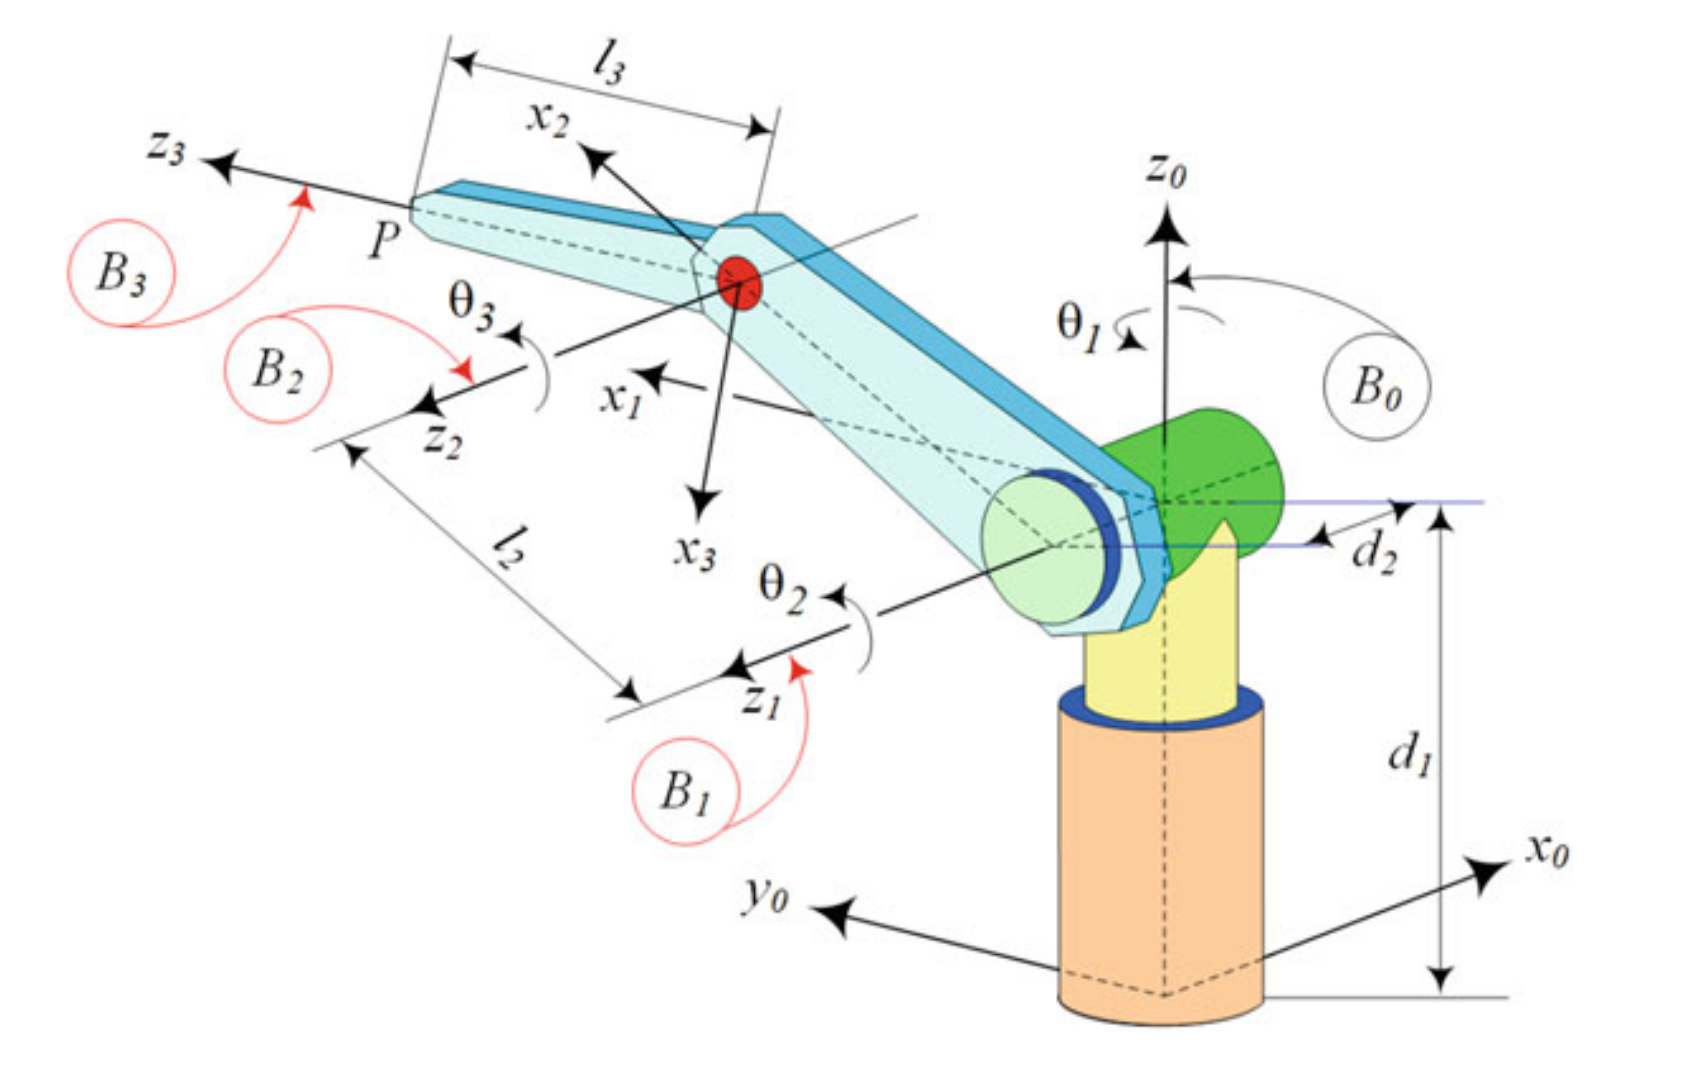
\includegraphics[width=\textwidth]{figures/articulated_arm.png}
            \captionof{figure}{A model of an articulated arm}
            \label{fig:articulated}
        \end{minipage}
        \hfill
        \begin{minipage}[b]{0.5\textwidth}
            \begin{tabular}{ c | c c c c }
                joint $i$ & $\theta_i$ & $d_i$ & $a_i$ & $\alpha_i$ \\ \hline
                1 & $\theta_1$ & $d_1$ & 0 & $- \frac{\pi}{2}$ \\
                2 & $\theta_2$ & $d_2$ &  $l_2$ & 0 \\
                3 & $\theta_3$ & $l_3$ &  0 & $\frac{\pi}{2}$ \\
            \end{tabular}
            \captionof{table}{DH parameter table for setting up the link frames}
            \label{tab:dhparam}
        \end{minipage}
    \end{figure}

    We want to compute the forward kinematics using the Denavit-Hartenberg convention. For that, the DH parameter table of the robot at rest position is set up as indicated in Table \ref{tab:dhparam}.

    % a) %%%%%%%%%%%%%%%%%% 
    \begin{subtask}[title=Forward Kinematics, points=4]{}
        Compute the transformations ${}^0 T_1$, ${}^1 T_2$ and then set up the forward kinematics model ${}^0 T_2$. \\
        
        \todo \\

    \end{subtask}{}
    
     % b) %%%%%%%%%%%%%%%%%% 
    \begin{subtask}[title=Trajectories, points=3]{}
        Please describe in words: What is a trajectory in robotics? Why should any trajectory representation be twice differentiable? Are cubic splines suitable for obtaining trajectories? \\

        \todo \\

    \end{subtask}{}
    
    % c) %%%%%%%%%%%%%%%%%% 
    \begin{subtask}[title=Differential Kinematics, points=4]{}
        Assume $x_\textrm{end-eff}=[x,y,z]^T$ (tip point \textbf{P}) given by:
    \[
        x_\textrm{end-eff} = {}^0 r_3 = \\
        \begin{pmatrix}
            ^0r_{3,x} \\
            ^0r_{3,y} \\
            ^0r_{3,z}
        \end{pmatrix} \\
        = \begin{pmatrix}
            -d_2 \, \sin \theta_1 + l_2 \, \cos \theta_1 \cos \theta_2 + l_3 \cos \theta_1 \sin (\theta_2 +\theta_3) \\
            d_2 \, \cos \theta_1 + l_2 \, \cos \theta_2 \sin \theta_1 + l_3 \sin \theta_1 \sin (\theta_2 +\theta_3) \\
            d_1 - l_2 \sin \theta_2 + l_3 \, \cos (\theta_2 +\theta_3)
        \end{pmatrix} 
    \]
    for the sake of simplicity, we additionally assume that $d_1 = d_2 = l_2 = l_3 = 1$. \\
    First, compute the Jacobian matrix $J(\theta)$ of the robot. Second, explain in a sentence the physical meaning of the Jacobian. \\
    \textbf{\textit{Hint:}} You can use the abbreviations $c(\theta)$ and $s(\theta)$ for $\cos(\theta)$ and $\sin(\theta)$ values. \\

        
        \todo \\

    \end{subtask}{}
    
    % d) %%%%%%%%%%%%%%%%%% 
    \begin{subtask}[title=Singularities, points=1]{}
        Please explain, what is a singularity in robotics? \\
        
        \todo \\
    
    
    \end{subtask}{}
    
    % e) %%%%%%%%%%%%%%%%%% 
    \begin{subtask}[title=[Bonus] Workspace, points=2]{}
        Sketch schematically a robot arm matching the workspace shown in figure \ref{fig:workspace_empty} with as few rotational and linear joints as possible. The origin of the coordinate system and the robot base are located at position $(0, 0)$ in the plot. Figure \ref{fig:robot_with_workspace_example} shows an example of the workspace of a $2$-DoF robot with $q_1$ rotational and $q_2$ linear joints.
        \begin{figure}[H]
            \centering
            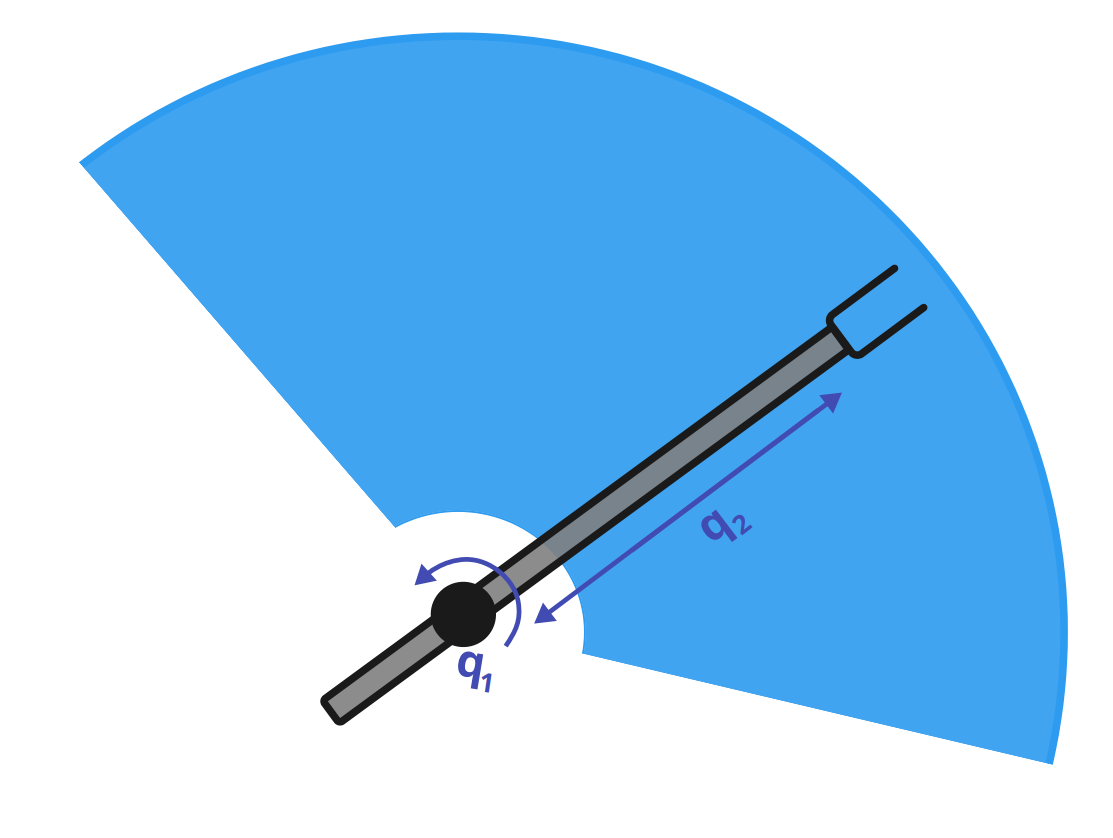
\includegraphics[width=0.5\textwidth]{figures/workspace_example.png}
            \captionof{figure}{An example of workspace for a robot with one rotational and one linear joint}
            \label{fig:robot_with_workspace_example}
        \end{figure} 
        
        \begin{figure}[H]
            \centering
            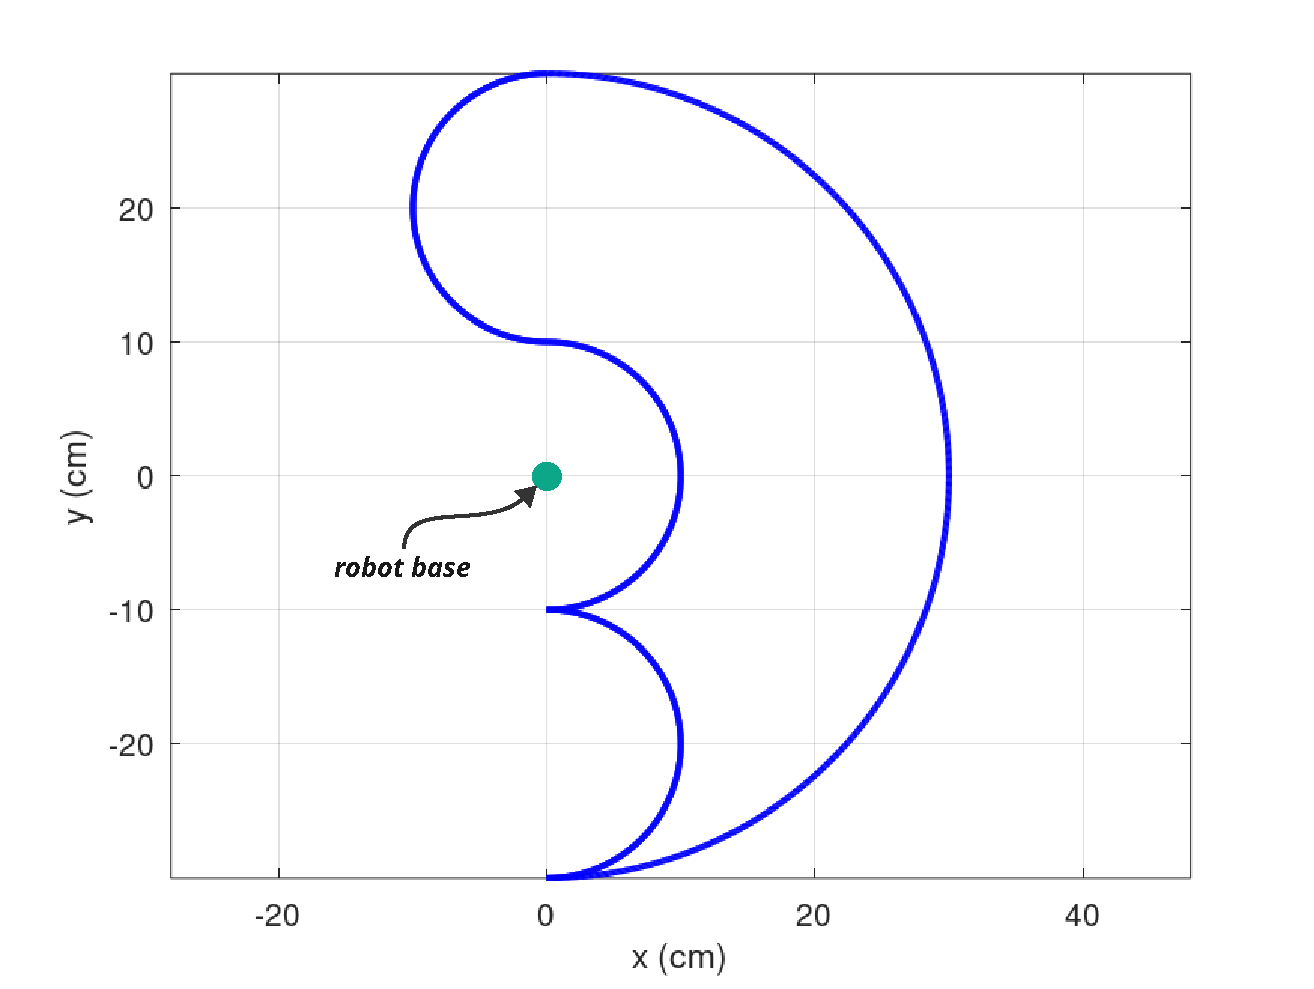
\includegraphics[width=0.7\textwidth]{figures/workspace_empty.pdf}
            \captionof{figure}{A workspace for a robot}
            \label{fig:workspace_empty}
        \end{figure}  
         
        \todo  
         
    \end{subtask}{}
    

    
\end{task}


%%%%%%%%%%%%%%%%%%%%%%%%%%%%%%%%%%%%%%%%%
%%%%%%%%%%%%%%%%%% 1.2 %%%%%%%%%%%%%%%%%% 
\begin{task}[points=30]{Control [+2 Bonus]} % 1.2
    In robotic locomotion it is common to abstract from the robot by using inverted pendulum models.
    In this exercise we will use a planar double inverted pendulum to test different control strategies. Our robot can be controlled by specifying the torque $\mathbf{u}=[u_1, u_2]$ of its motors. Consider that in mechanical systems the torque $u$ is a function of the joint positions $q$, velocities $\dot{q}$ and accelerations $\ddot{q}$, as given by  
    \[
        u=M(q)\ddot{q}+c(q,\dot{q})+g(q), 
    \] 
    where $M$ denotes the inertial matrix, $c(q,\dot{q})$ the Coriolis and centripetal forces, and $g$ the gravity terms.

    \textbf{For the programming part of this exercise (starting from question b))}, you will use the code that is attached to the exercise.
    The code is organized as follows: By commenting / uncommenting the specific lines in \texttt{example.py} you can choose which controller configuration to run. Already after downloading the files, running \texttt{example.py} should generate some plots, however, without the robot moving at all as the controllers currently just apply a constant action of all zeros. Thus, you have to modify the controllers, inside \texttt{my\_ctrl.py} (for b), c), d)), and inside \texttt{my\_taskSpace\_ctrl.py} for the last part. If you want to dive deeper into the code, you can start from \texttt{my\_ctl.py} / \texttt{my\_taskSpace\_ctl.py}.
    Please attach figures of the plots that you generated in here, and provide short snippets of your code! Also, please submit your code with the exercise. Note: please leave all the files unchanged and only modify \texttt{example.py} (commenting / uncommenting depending on which configuration you want to run), as well as \texttt{my\_ctrl.py} and \texttt{my\_taskSpace\_ctrl.py}.

    
    % a) %%%%%%%%%%%%%%%%%% 
    \begin{subtask}[title=Gravity Compensation and Inverse Dynamics Control, points=5]{}
        Suppose that you would like to create a control law to set the joint angles on the double inverted pendulum model by controlling the torque of the motors. First, provide a PD-feedback control law which additionally compensates for gravity. Second, extend the previous control law to full inverse dynamics control. Lastly, will the PD control law with gravity compensation perfectly reach a desired setpoint when having an imperfect
robot model? \\
        
        \todo \\

    \end{subtask}  
    
    % b) %%%%%%%%%%%%%%%%%% 
    \begin{subtask}[title=Comparison of Different Control Strategies, points=15]{}
		In the following exercise you will investigate the differences of the following control algorithms, P, PD, PID, PD with gravity compensation, and full inverse dynamics.
		The double pendulum is initiated hanging down, with state $q_\textrm{start}={[-\pi,0]}$. We simulate the system with a time-step $dt=0.002$ seconds using symplectic Euler integration and run the simulation for $t_\textrm{end}=3s$. 

		Implement the control laws by filling the skeleton file \texttt{my\_ctl.py}. Use the following feedback gains $K_P=65, K_D=12, K_I=0.1$ for the first joint and $K_P=35, K_D=8, K_I=0.1$ for the second one.
		The target state of the double pendulum is set to $q_\textrm{des}={[-\pi / 2,0]}$.

		Create plots that compare the different control strategies and analyze the results. It is your choice how to illustrate your results. However, we already provide code to generate the plots, which is sufficient. We thus stronly advise to leave the code untouched (this also makes correction way easier, when we re-run the code that you submitted). Do not forget to include your source code in your solutions. \\
		To modify and/or run the code, see the "Additional Information" section in the README file. \\

        \todo \\

    \end{subtask}  
    
    % c) %%%%%%%%%%%%%%%%%% 
    \begin{subtask}[title=Tracking Trajectories, points=5]{}
        Repeat the same experiment but this time use the provided time-varying target trajectory. Create plots that compare the different control strategies and analyze the results. \\
        
        \todo \\

    \end{subtask}    
    
    % d) %%%%%%%%%%%%%%%%%% 
    \begin{subtask}[title= [Bonus] Tracking Trajectories — High Gains, points=2]{}
        Repeat the previous experiment for the PD controller, but now with all gains multiplied by 5. What do you observe? Are there any drawbacks of using high gains? \\
        
        \todo \\

    \end{subtask}  
    

    % e) %%%%%%%%%%%%%%%%%% 
    \begin{subtask}[title=Task Space Control, points=5]{}
        The robot must now reach a desired position in task space $x_\textrm{end}={[0.0,1.2]}$. In class we derived the Jacobian transpose, Jacobian pseudo-inverse, and Jacobian pseudo-inverse with damping methods. All of them are implemented in \texttt{my\_taskSpace\_ctl.py}. You are asked to implement also the null-space task prioritization method with a null-space resting posture $q=[0,\pi]$. Run the simulation and plot the initial and final configuration of the robot. Then, change the resting posture to $q=[0,-\pi]$ and redo the plots. Analyze in a couple of sentences your observation. Use the same damping coefficient $10^{-6}$ and include a code snippet to your solutions. \\
        
        \todo \\
        
    \end{subtask} 
    
    
\end{task}




\end{document}
